\begin{figure}[t]
\centering
\begin{tabular}{c}
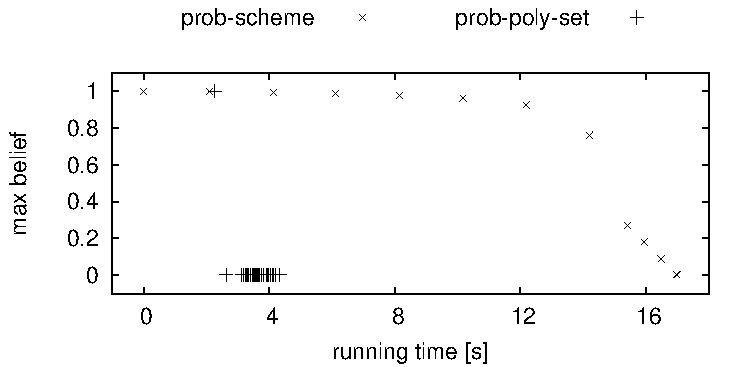
\includegraphics[width=9cm]{figures/plot_bday.pdf} \\
(a) birthday query (\eref{ex:bday}) \\
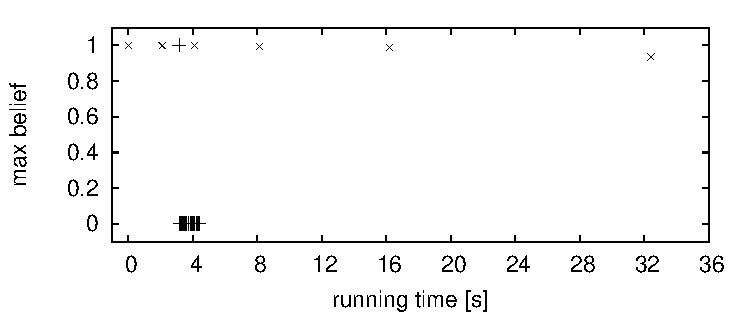
\includegraphics[width=9cm]{figures/plot_bday_large.pdf} \\
(b) birthday query (\eref{ex:bday}), larger state space \\
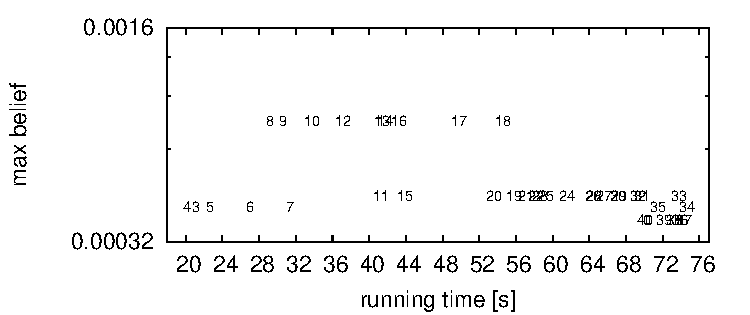
\includegraphics[width=9cm]{figures/plot_bday_seq.pdf} \\
(c) special year query (\eref{ex:specyear}) \\
\end{tabular}
\caption{Query evaluation comparison}
\label{fig:plots_bday}
\end{figure}

\iffull
\begin{table*}[t]
\scriptsize
\centering
\begin{tabular}{||p{1.35cm}|p{0.50cm}p{0.50cm}p{0.50cm}p{0.50cm}p{0.50cm}p{0.50cm}p{0.50cm}p{0.50cm}p{0.50cm}p{0.50cm}p{0.50cm}p{0.50cm}p{0.50cm}p{0.50cm}p{0.50cm}p{0.50cm}p{0.50cm}c||}
\hline \hline {\small time [s]} \par {\scriptsize max belief}& \multicolumn{18}{c||}{\textbf{prob-poly set size bound}} \\
\hline \hline \textbf{query} & \textbf{1} & \textbf{2} & \textbf{3} & \textbf{4} & \textbf{5} & \textbf{6} & \textbf{7} & \textbf{8} & \textbf{9} & \textbf{10} & \textbf{15} & \textbf{20} & \textbf{25} & \textbf{30} & \textbf{35} & \textbf{40} & \textbf{$ \infty $} & \\
\hline \hline bday \par 1 box & {\small 0.0}\par{\scriptsize\parbox{1.0cm}{1}} \par{\scriptsize 0} & {\small 0.0}\par{\scriptsize\parbox{1.0cm}{0.00386}} \par{\scriptsize 0} & {\small 0.0}\par{\scriptsize\parbox{1.0cm}{0.00386}} \par{\scriptsize 0} & {\small 0.0}\par{\scriptsize\parbox{1.0cm}{0.00386}} \par{\scriptsize 0} & {\small 0.0}\par{\scriptsize\parbox{1.0cm}{0.00386}} \par{\scriptsize 0} & {\small 0.0}\par{\scriptsize\parbox{1.0cm}{0.00386}} \par{\scriptsize 0} & {\small 0.0}\par{\scriptsize\parbox{1.0cm}{0.00386}} \par{\scriptsize 0} & {\small 0.0}\par{\scriptsize\parbox{1.0cm}{0.00386}} \par{\scriptsize 0} & {\small 0.0}\par{\scriptsize\parbox{1.0cm}{0.00386}} \par{\scriptsize 0} & {\small 0.0}\par{\scriptsize\parbox{1.0cm}{0.00386}} \par{\scriptsize 0} & {\small 0.0}\par{\scriptsize\parbox{1.0cm}{0.00386}} \par{\scriptsize 0} & {\small 0.0}\par{\scriptsize\parbox{1.0cm}{0.00386}} \par{\scriptsize 0} & {\small 0.0}\par{\scriptsize\parbox{1.0cm}{0.00386}} \par{\scriptsize 0} & {\small 0.0}\par{\scriptsize\parbox{1.0cm}{0.00386}} \par{\scriptsize 0} & {\small 0.0}\par{\scriptsize\parbox{1.0cm}{0.00386}} \par{\scriptsize 0} & {\small 0.0}\par{\scriptsize\parbox{1.0cm}{0.00386}} \par{\scriptsize 0} & {\small 0.0}\par{\scriptsize\parbox{1.0cm}{0.00386}} \par{\scriptsize 0} & \\
\hline bday \par 1 octalatte & {\small 0.6}\par{\scriptsize\parbox{1.0cm}{1}} \par{\scriptsize 8} & {\small 0.6}\par{\scriptsize\parbox{1.0cm}{0.00386}} \par{\scriptsize 8} & {\small 0.7}\par{\scriptsize\parbox{1.0cm}{0.00386}} \par{\scriptsize 8} & {\small 0.7}\par{\scriptsize\parbox{1.0cm}{0.00386}} \par{\scriptsize 8} & {\small 0.7}\par{\scriptsize\parbox{1.0cm}{0.00386}} \par{\scriptsize 8} & {\small 0.7}\par{\scriptsize\parbox{1.0cm}{0.00386}} \par{\scriptsize 8} & {\small 0.7}\par{\scriptsize\parbox{1.0cm}{0.00386}} \par{\scriptsize 8} & {\small 0.8}\par{\scriptsize\parbox{1.0cm}{0.00386}} \par{\scriptsize 8} & {\small 0.7}\par{\scriptsize\parbox{1.0cm}{0.00386}} \par{\scriptsize 8} & {\small 0.7}\par{\scriptsize\parbox{1.0cm}{0.00386}} \par{\scriptsize 8} & {\small 0.9}\par{\scriptsize\parbox{1.0cm}{0.00386}} \par{\scriptsize 8} & {\small 0.7}\par{\scriptsize\parbox{1.0cm}{0.00386}} \par{\scriptsize 8} & {\small 0.7}\par{\scriptsize\parbox{1.0cm}{0.00386}} \par{\scriptsize 8} & {\small 0.8}\par{\scriptsize\parbox{1.0cm}{0.00386}} \par{\scriptsize 8} & {\small 0.8}\par{\scriptsize\parbox{1.0cm}{0.00386}} \par{\scriptsize 8} & {\small 0.7}\par{\scriptsize\parbox{1.0cm}{0.00386}} \par{\scriptsize 8} & {\small 0.7}\par{\scriptsize\parbox{1.0cm}{0.00386}} \par{\scriptsize 8} & \\
\hline bday \par 1 poly & {\small 0.7}\par{\scriptsize\parbox{1.0cm}{1}} \par{\scriptsize 8} & {\small 0.7}\par{\scriptsize\parbox{1.0cm}{0.00386}} \par{\scriptsize 8} & {\small 0.8}\par{\scriptsize\parbox{1.0cm}{0.00386}} \par{\scriptsize 8} & {\small 0.9}\par{\scriptsize\parbox{1.0cm}{0.00386}} \par{\scriptsize 8} & {\small 0.8}\par{\scriptsize\parbox{1.0cm}{0.00386}} \par{\scriptsize 8} & {\small 0.8}\par{\scriptsize\parbox{1.0cm}{0.00386}} \par{\scriptsize 8} & {\small 0.8}\par{\scriptsize\parbox{1.0cm}{0.00386}} \par{\scriptsize 8} & {\small 0.8}\par{\scriptsize\parbox{1.0cm}{0.00386}} \par{\scriptsize 8} & {\small 0.8}\par{\scriptsize\parbox{1.0cm}{0.00386}} \par{\scriptsize 8} & {\small 0.8}\par{\scriptsize\parbox{1.0cm}{0.00386}} \par{\scriptsize 8} & {\small 0.8}\par{\scriptsize\parbox{1.0cm}{0.00386}} \par{\scriptsize 8} & {\small 0.9}\par{\scriptsize\parbox{1.0cm}{0.00386}} \par{\scriptsize 8} & {\small 0.9}\par{\scriptsize\parbox{1.0cm}{0.00386}} \par{\scriptsize 8} & {\small 0.8}\par{\scriptsize\parbox{1.0cm}{0.00386}} \par{\scriptsize 8} & {\small 0.8}\par{\scriptsize\parbox{1.0cm}{0.00386}} \par{\scriptsize 8} & {\small 0.8}\par{\scriptsize\parbox{1.0cm}{0.00386}} \par{\scriptsize 8} & {\small 0.8}\par{\scriptsize\parbox{1.0cm}{0.00386}} \par{\scriptsize 8} & \\
\hline bday \par 1+2 box & {\small 0.0}\par{\scriptsize\parbox{1.0cm}{1}} \par{\scriptsize 0} & {\small 0.0}\par{\scriptsize\parbox{1.0cm}{1}} \par{\scriptsize 0} & {\small 0.0}\par{\scriptsize\parbox{1.0cm}{0.02703}} \par{\scriptsize 0} & {\small 0.0}\par{\scriptsize\parbox{1.0cm}{0.02703}} \par{\scriptsize 0} & {\small 0.0}\par{\scriptsize\parbox{1.0cm}{0.02703}} \par{\scriptsize 0} & {\small 0.0}\par{\scriptsize\parbox{1.0cm}{0.02703}} \par{\scriptsize 0} & {\small 0.0}\par{\scriptsize\parbox{1.0cm}{0.02703}} \par{\scriptsize 0} & {\small 0.0}\par{\scriptsize\parbox{1.0cm}{0.02703}} \par{\scriptsize 0} & {\small 0.0}\par{\scriptsize\parbox{1.0cm}{0.02703}} \par{\scriptsize 0} & {\small 0.0}\par{\scriptsize\parbox{1.0cm}{0.02703}} \par{\scriptsize 0} & {\small 0.0}\par{\scriptsize\parbox{1.0cm}{0.02703}} \par{\scriptsize 0} & {\small 0.0}\par{\scriptsize\parbox{1.0cm}{0.02703}} \par{\scriptsize 0} & {\small 0.0}\par{\scriptsize\parbox{1.0cm}{0.02703}} \par{\scriptsize 0} & {\small 0.0}\par{\scriptsize\parbox{1.0cm}{0.02703}} \par{\scriptsize 0} & {\small 0.0}\par{\scriptsize\parbox{1.0cm}{0.02703}} \par{\scriptsize 0} & {\small 0.0}\par{\scriptsize\parbox{1.0cm}{0.02703}} \par{\scriptsize 0} & {\small 0.0}\par{\scriptsize\parbox{1.0cm}{0.02703}} \par{\scriptsize 0} & \\
\hline bday \par 1+2 octalatte & {\small 0.8}\par{\scriptsize\parbox{1.0cm}{1}} \par{\scriptsize 6} & {\small 1.3}\par{\scriptsize\parbox{1.0cm}{1}} \par{\scriptsize 8} & {\small 1.4}\par{\scriptsize\parbox{1.0cm}{0.02703}} \par{\scriptsize 8} & {\small 1.4}\par{\scriptsize\parbox{1.0cm}{0.02703}} \par{\scriptsize 8} & {\small 1.5}\par{\scriptsize\parbox{1.0cm}{0.02703}} \par{\scriptsize 8} & {\small 1.5}\par{\scriptsize\parbox{1.0cm}{0.02703}} \par{\scriptsize 8} & {\small 1.5}\par{\scriptsize\parbox{1.0cm}{0.02703}} \par{\scriptsize 8} & {\small 2.1}\par{\scriptsize\parbox{1.0cm}{0.02703}} \par{\scriptsize 8} & {\small 1.5}\par{\scriptsize\parbox{1.0cm}{0.02703}} \par{\scriptsize 8} & {\small 2.4}\par{\scriptsize\parbox{1.0cm}{0.02703}} \par{\scriptsize 8} & {\small 1.7}\par{\scriptsize\parbox{1.0cm}{0.02703}} \par{\scriptsize 8} & {\small 1.5}\par{\scriptsize\parbox{1.0cm}{0.02703}} \par{\scriptsize 8} & {\small 1.5}\par{\scriptsize\parbox{1.0cm}{0.02703}} \par{\scriptsize 8} & {\small 1.5}\par{\scriptsize\parbox{1.0cm}{0.02703}} \par{\scriptsize 8} & {\small 1.5}\par{\scriptsize\parbox{1.0cm}{0.02703}} \par{\scriptsize 8} & {\small 1.4}\par{\scriptsize\parbox{1.0cm}{0.02703}} \par{\scriptsize 8} & {\small 1.5}\par{\scriptsize\parbox{1.0cm}{0.02703}} \par{\scriptsize 8} & \\
\hline bday \par 1+2 poly & {\small 1.1}\par{\scriptsize\parbox{1.0cm}{1}} \par{\scriptsize 8} & {\small 1.3}\par{\scriptsize\parbox{1.0cm}{1}} \par{\scriptsize 8} & {\small 1.6}\par{\scriptsize\parbox{1.0cm}{0.02703}} \par{\scriptsize 8} & {\small 2.6}\par{\scriptsize\parbox{1.0cm}{0.02703}} \par{\scriptsize 8} & {\small 1.6}\par{\scriptsize\parbox{1.0cm}{0.02703}} \par{\scriptsize 8} & {\small 1.6}\par{\scriptsize\parbox{1.0cm}{0.02703}} \par{\scriptsize 8} & {\small 1.6}\par{\scriptsize\parbox{1.0cm}{0.02703}} \par{\scriptsize 8} & {\small 1.6}\par{\scriptsize\parbox{1.0cm}{0.02703}} \par{\scriptsize 8} & {\small 1.6}\par{\scriptsize\parbox{1.0cm}{0.02703}} \par{\scriptsize 8} & {\small 1.6}\par{\scriptsize\parbox{1.0cm}{0.02703}} \par{\scriptsize 8} & {\small 1.6}\par{\scriptsize\parbox{1.0cm}{0.02703}} \par{\scriptsize 8} & {\small 1.6}\par{\scriptsize\parbox{1.0cm}{0.02703}} \par{\scriptsize 8} & {\small 1.6}\par{\scriptsize\parbox{1.0cm}{0.02703}} \par{\scriptsize 8} & {\small 1.7}\par{\scriptsize\parbox{1.0cm}{0.02703}} \par{\scriptsize 8} & {\small 1.6}\par{\scriptsize\parbox{1.0cm}{0.02703}} \par{\scriptsize 8} & {\small 1.6}\par{\scriptsize\parbox{1.0cm}{0.02703}} \par{\scriptsize 8} & {\small 1.6}\par{\scriptsize\parbox{1.0cm}{0.02703}} \par{\scriptsize 8} & \\
\hline bday \par 1+2+special box & {\small 0.5}\par{\scriptsize\parbox{1.0cm}{1}} \par{\scriptsize 0} & {\small 0.5}\par{\scriptsize\parbox{1.0cm}{1}} \par{\scriptsize 0} & {\small 0.4}\par{\scriptsize\parbox{1.0cm}{4.22e-4}} \par{\scriptsize 0} & {\small 0.4}\par{\scriptsize\parbox{1.0cm}{4.22e-4}} \par{\scriptsize 0} & {\small 0.4}\par{\scriptsize\parbox{1.0cm}{4.22e-4}} \par{\scriptsize 0} & {\small 0.4}\par{\scriptsize\parbox{1.0cm}{4.22e-4}} \par{\scriptsize 0} & {\small 0.4}\par{\scriptsize\parbox{1.0cm}{4.22e-4}} \par{\scriptsize 0} & {\small 0.4}\par{\scriptsize\parbox{1.0cm}{8.06e-4}} \par{\scriptsize 0} & {\small 0.4}\par{\scriptsize\parbox{1.0cm}{8.06e-4}} \par{\scriptsize 0} & {\small 0.5}\par{\scriptsize\parbox{1.0cm}{8.06e-4}} \par{\scriptsize 0} & {\small 0.5}\par{\scriptsize\parbox{1.0cm}{4.60e-4}} \par{\scriptsize 0} & {\small 0.5}\par{\scriptsize\parbox{1.0cm}{0.00186}} \par{\scriptsize 0} & {\small 0.5}\par{\scriptsize\parbox{1.0cm}{0.00163}} \par{\scriptsize 0} & {\small 0.5}\par{\scriptsize\parbox{1.0cm}{0.00145}} \par{\scriptsize 0} & {\small 0.5}\par{\scriptsize\parbox{1.0cm}{4.60e-4}} \par{\scriptsize 0} & {\small 0.5}\par{\scriptsize\parbox{1.0cm}{3.84e-4}} \par{\scriptsize 0} & {\small 0.5}\par{\scriptsize\parbox{1.0cm}{3.84e-4}} \par{\scriptsize 0} & \\
\hline bday \par 1+2+special octalatte & {\small 2.7}\par{\scriptsize\parbox{1.0cm}{1}} \par{\scriptsize 10} & {\small 3.7}\par{\scriptsize\parbox{1.0cm}{1}} \par{\scriptsize 12} & {\small 8.0}\par{\scriptsize\parbox{1.0cm}{4.22e-4}} \par{\scriptsize 12} & {\small 5.0}\par{\scriptsize\parbox{1.0cm}{4.22e-4}} \par{\scriptsize 10} & {\small 7.2}\par{\scriptsize\parbox{1.0cm}{4.22e-4}} \par{\scriptsize 11} & {\small 5.9}\par{\scriptsize\parbox{1.0cm}{4.22e-4}} \par{\scriptsize 11} & {\small 6.7}\par{\scriptsize\parbox{1.0cm}{4.22e-4}} \par{\scriptsize 11} & {\small 8.0}\par{\scriptsize\parbox{1.0cm}{8.06e-4}} \par{\scriptsize 11} & {\small 7.0}\par{\scriptsize\parbox{1.0cm}{8.06e-4}} \par{\scriptsize 11} & {\small 10.7}\par{\scriptsize\parbox{1.0cm}{8.06e-4}} \par{\scriptsize 11} & {\small 12.4}\par{\scriptsize\parbox{1.0cm}{4.60e-4}} \par{\scriptsize 11} & {\small 14.7}\par{\scriptsize\parbox{1.0cm}{0.00132}} \par{\scriptsize 16} & {\small 14.9}\par{\scriptsize\parbox{1.0cm}{0.00116}} \par{\scriptsize 16} & {\small 15.9}\par{\scriptsize\parbox{1.0cm}{0.00103}} \par{\scriptsize 16} & {\small 15.3}\par{\scriptsize\parbox{1.0cm}{4.60e-4}} \par{\scriptsize 14} & {\small 17.2}\par{\scriptsize\parbox{1.0cm}{3.84e-4}} \par{\scriptsize 10} & {\small 16.1}\par{\scriptsize\parbox{1.0cm}{3.84e-4}} \par{\scriptsize 10} & \\
\hline bday \par 1+2+special poly & {\small 3.4}\par{\scriptsize\parbox{1.0cm}{1}} \par{\scriptsize 10} & {\small 5.7}\par{\scriptsize\parbox{1.0cm}{1}} \par{\scriptsize 12} & {\small 5.0}\par{\scriptsize\parbox{1.0cm}{4.22e-4}} \par{\scriptsize 12} & {\small 6.3}\par{\scriptsize\parbox{1.0cm}{4.22e-4}} \par{\scriptsize 10} & {\small 8.7}\par{\scriptsize\parbox{1.0cm}{4.22e-4}} \par{\scriptsize 11} & {\small 6.0}\par{\scriptsize\parbox{1.0cm}{4.22e-4}} \par{\scriptsize 11} & {\small 6.8}\par{\scriptsize\parbox{1.0cm}{4.22e-4}} \par{\scriptsize 11} & {\small 10.8}\par{\scriptsize\parbox{1.0cm}{8.06e-4}} \par{\scriptsize 11} & {\small 8.7}\par{\scriptsize\parbox{1.0cm}{8.06e-4}} \par{\scriptsize 11} & {\small 7.4}\par{\scriptsize\parbox{1.0cm}{8.06e-4}} \par{\scriptsize 11} & {\small 10.9}\par{\scriptsize\parbox{1.0cm}{4.60e-4}} \par{\scriptsize 11} & {\small 14.2}\par{\scriptsize\parbox{1.0cm}{4.60e-4}} \par{\scriptsize 14} & {\small 16.9}\par{\scriptsize\parbox{1.0cm}{4.60e-4}} \par{\scriptsize 14} & {\small 18.2}\par{\scriptsize\parbox{1.0cm}{4.60e-4}} \par{\scriptsize 14} & {\small 18.5}\par{\scriptsize\parbox{1.0cm}{4.22e-4}} \par{\scriptsize 12} & {\small 18.0}\par{\scriptsize\parbox{1.0cm}{3.84e-4}} \par{\scriptsize 10} & {\small 18.2}\par{\scriptsize\parbox{1.0cm}{3.84e-4}} \par{\scriptsize 10} & \\
\hline \hline bday large \par 1 box & {\small 0.0}\par{\scriptsize\parbox{1.0cm}{1}} \par{\scriptsize 0} & {\small 0.0}\par{\scriptsize\parbox{1.0cm}{0.00141}} \par{\scriptsize 0} & {\small 0.0}\par{\scriptsize\parbox{1.0cm}{0.00141}} \par{\scriptsize 0} & {\small 0.0}\par{\scriptsize\parbox{1.0cm}{0.00141}} \par{\scriptsize 0} & {\small 0.0}\par{\scriptsize\parbox{1.0cm}{0.00141}} \par{\scriptsize 0} & {\small 0.0}\par{\scriptsize\parbox{1.0cm}{0.00141}} \par{\scriptsize 0} & {\small 0.0}\par{\scriptsize\parbox{1.0cm}{0.00141}} \par{\scriptsize 0} & {\small 0.0}\par{\scriptsize\parbox{1.0cm}{0.00141}} \par{\scriptsize 0} & {\small 0.0}\par{\scriptsize\parbox{1.0cm}{0.00141}} \par{\scriptsize 0} & {\small 0.0}\par{\scriptsize\parbox{1.0cm}{0.00141}} \par{\scriptsize 0} & {\small 0.0}\par{\scriptsize\parbox{1.0cm}{0.00141}} \par{\scriptsize 0} & {\small 0.0}\par{\scriptsize\parbox{1.0cm}{0.00141}} \par{\scriptsize 0} & {\small 0.0}\par{\scriptsize\parbox{1.0cm}{0.00141}} \par{\scriptsize 0} & {\small 0.0}\par{\scriptsize\parbox{1.0cm}{0.00141}} \par{\scriptsize 0} & {\small 0.0}\par{\scriptsize\parbox{1.0cm}{0.00141}} \par{\scriptsize 0} & {\small 0.0}\par{\scriptsize\parbox{1.0cm}{0.00141}} \par{\scriptsize 0} & {\small 0.0}\par{\scriptsize\parbox{1.0cm}{0.00141}} \par{\scriptsize 0} & \\
\hline bday large \par 1 octalatte & {\small 0.6}\par{\scriptsize\parbox{1.0cm}{1}} \par{\scriptsize 8} & {\small 0.6}\par{\scriptsize\parbox{1.0cm}{0.00141}} \par{\scriptsize 8} & {\small 0.8}\par{\scriptsize\parbox{1.0cm}{0.00141}} \par{\scriptsize 8} & {\small 0.8}\par{\scriptsize\parbox{1.0cm}{0.00141}} \par{\scriptsize 8} & {\small 0.7}\par{\scriptsize\parbox{1.0cm}{0.00141}} \par{\scriptsize 8} & {\small 0.8}\par{\scriptsize\parbox{1.0cm}{0.00141}} \par{\scriptsize 8} & {\small 0.7}\par{\scriptsize\parbox{1.0cm}{0.00141}} \par{\scriptsize 8} & {\small 0.7}\par{\scriptsize\parbox{1.0cm}{0.00141}} \par{\scriptsize 8} & {\small 0.7}\par{\scriptsize\parbox{1.0cm}{0.00141}} \par{\scriptsize 8} & {\small 0.7}\par{\scriptsize\parbox{1.0cm}{0.00141}} \par{\scriptsize 8} & {\small 1.7}\par{\scriptsize\parbox{1.0cm}{0.00141}} \par{\scriptsize 8} & {\small 0.7}\par{\scriptsize\parbox{1.0cm}{0.00141}} \par{\scriptsize 8} & {\small 0.7}\par{\scriptsize\parbox{1.0cm}{0.00141}} \par{\scriptsize 8} & {\small 0.7}\par{\scriptsize\parbox{1.0cm}{0.00141}} \par{\scriptsize 8} & {\small 0.7}\par{\scriptsize\parbox{1.0cm}{0.00141}} \par{\scriptsize 8} & {\small 0.7}\par{\scriptsize\parbox{1.0cm}{0.00141}} \par{\scriptsize 8} & {\small 0.8}\par{\scriptsize\parbox{1.0cm}{0.00141}} \par{\scriptsize 8} & \\
\hline bday large \par 1 poly & {\small 0.7}\par{\scriptsize\parbox{1.0cm}{1}} \par{\scriptsize 8} & {\small 0.7}\par{\scriptsize\parbox{1.0cm}{0.00141}} \par{\scriptsize 8} & {\small 0.8}\par{\scriptsize\parbox{1.0cm}{0.00141}} \par{\scriptsize 8} & {\small 0.9}\par{\scriptsize\parbox{1.0cm}{0.00141}} \par{\scriptsize 8} & {\small 0.8}\par{\scriptsize\parbox{1.0cm}{0.00141}} \par{\scriptsize 8} & {\small 0.8}\par{\scriptsize\parbox{1.0cm}{0.00141}} \par{\scriptsize 8} & {\small 0.9}\par{\scriptsize\parbox{1.0cm}{0.00141}} \par{\scriptsize 8} & {\small 0.9}\par{\scriptsize\parbox{1.0cm}{0.00141}} \par{\scriptsize 8} & {\small 1.5}\par{\scriptsize\parbox{1.0cm}{0.00141}} \par{\scriptsize 8} & {\small 0.9}\par{\scriptsize\parbox{1.0cm}{0.00141}} \par{\scriptsize 8} & {\small 0.8}\par{\scriptsize\parbox{1.0cm}{0.00141}} \par{\scriptsize 8} & {\small 0.8}\par{\scriptsize\parbox{1.0cm}{0.00141}} \par{\scriptsize 8} & {\small 0.9}\par{\scriptsize\parbox{1.0cm}{0.00141}} \par{\scriptsize 8} & {\small 0.8}\par{\scriptsize\parbox{1.0cm}{0.00141}} \par{\scriptsize 8} & {\small 0.9}\par{\scriptsize\parbox{1.0cm}{0.00141}} \par{\scriptsize 8} & {\small 0.8}\par{\scriptsize\parbox{1.0cm}{0.00141}} \par{\scriptsize 8} & {\small 0.8}\par{\scriptsize\parbox{1.0cm}{0.00141}} \par{\scriptsize 8} & \\
\hline bday large \par 1+2 box & {\small 0.0}\par{\scriptsize\parbox{1.0cm}{1}} \par{\scriptsize 0} & {\small 0.0}\par{\scriptsize\parbox{1.0cm}{1}} \par{\scriptsize 0} & {\small 0.0}\par{\scriptsize\parbox{1.0cm}{0.00990}} \par{\scriptsize 0} & {\small 0.0}\par{\scriptsize\parbox{1.0cm}{0.00990}} \par{\scriptsize 0} & {\small 0.0}\par{\scriptsize\parbox{1.0cm}{0.00990}} \par{\scriptsize 0} & {\small 0.0}\par{\scriptsize\parbox{1.0cm}{0.00990}} \par{\scriptsize 0} & {\small 0.0}\par{\scriptsize\parbox{1.0cm}{0.00990}} \par{\scriptsize 0} & {\small 0.0}\par{\scriptsize\parbox{1.0cm}{0.00990}} \par{\scriptsize 0} & {\small 0.0}\par{\scriptsize\parbox{1.0cm}{0.00990}} \par{\scriptsize 0} & {\small 0.0}\par{\scriptsize\parbox{1.0cm}{0.00990}} \par{\scriptsize 0} & {\small 0.0}\par{\scriptsize\parbox{1.0cm}{0.00990}} \par{\scriptsize 0} & {\small 0.0}\par{\scriptsize\parbox{1.0cm}{0.00990}} \par{\scriptsize 0} & {\small 0.0}\par{\scriptsize\parbox{1.0cm}{0.00990}} \par{\scriptsize 0} & {\small 0.0}\par{\scriptsize\parbox{1.0cm}{0.00990}} \par{\scriptsize 0} & {\small 0.0}\par{\scriptsize\parbox{1.0cm}{0.00990}} \par{\scriptsize 0} & {\small 0.0}\par{\scriptsize\parbox{1.0cm}{0.00990}} \par{\scriptsize 0} & {\small 0.0}\par{\scriptsize\parbox{1.0cm}{0.00990}} \par{\scriptsize 0} & \\
\hline bday large \par 1+2 octalatte & {\small 0.8}\par{\scriptsize\parbox{1.0cm}{1}} \par{\scriptsize 6} & {\small 1.3}\par{\scriptsize\parbox{1.0cm}{1}} \par{\scriptsize 8} & {\small 1.5}\par{\scriptsize\parbox{1.0cm}{0.00990}} \par{\scriptsize 8} & {\small 1.5}\par{\scriptsize\parbox{1.0cm}{0.00990}} \par{\scriptsize 8} & {\small 1.4}\par{\scriptsize\parbox{1.0cm}{0.00990}} \par{\scriptsize 8} & {\small 1.5}\par{\scriptsize\parbox{1.0cm}{0.00990}} \par{\scriptsize 8} & {\small 1.5}\par{\scriptsize\parbox{1.0cm}{0.00990}} \par{\scriptsize 8} & {\small 1.5}\par{\scriptsize\parbox{1.0cm}{0.00990}} \par{\scriptsize 8} & {\small 1.5}\par{\scriptsize\parbox{1.0cm}{0.00990}} \par{\scriptsize 8} & {\small 1.4}\par{\scriptsize\parbox{1.0cm}{0.00990}} \par{\scriptsize 8} & {\small 3.0}\par{\scriptsize\parbox{1.0cm}{0.00990}} \par{\scriptsize 8} & {\small 1.5}\par{\scriptsize\parbox{1.0cm}{0.00990}} \par{\scriptsize 8} & {\small 1.4}\par{\scriptsize\parbox{1.0cm}{0.00990}} \par{\scriptsize 8} & {\small 1.4}\par{\scriptsize\parbox{1.0cm}{0.00990}} \par{\scriptsize 8} & {\small 1.4}\par{\scriptsize\parbox{1.0cm}{0.00990}} \par{\scriptsize 8} & {\small 1.4}\par{\scriptsize\parbox{1.0cm}{0.00990}} \par{\scriptsize 8} & {\small 1.5}\par{\scriptsize\parbox{1.0cm}{0.00990}} \par{\scriptsize 8} & \\
\hline bday large \par 1+2 poly & {\small 1.1}\par{\scriptsize\parbox{1.0cm}{1}} \par{\scriptsize 8} & {\small 1.3}\par{\scriptsize\parbox{1.0cm}{1}} \par{\scriptsize 8} & {\small 1.6}\par{\scriptsize\parbox{1.0cm}{0.00990}} \par{\scriptsize 8} & {\small 1.6}\par{\scriptsize\parbox{1.0cm}{0.00990}} \par{\scriptsize 8} & {\small 1.6}\par{\scriptsize\parbox{1.0cm}{0.00990}} \par{\scriptsize 8} & {\small 1.6}\par{\scriptsize\parbox{1.0cm}{0.00990}} \par{\scriptsize 8} & {\small 1.6}\par{\scriptsize\parbox{1.0cm}{0.00990}} \par{\scriptsize 8} & {\small 1.6}\par{\scriptsize\parbox{1.0cm}{0.00990}} \par{\scriptsize 8} & {\small 3.1}\par{\scriptsize\parbox{1.0cm}{0.00990}} \par{\scriptsize 8} & {\small 1.7}\par{\scriptsize\parbox{1.0cm}{0.00990}} \par{\scriptsize 8} & {\small 1.6}\par{\scriptsize\parbox{1.0cm}{0.00990}} \par{\scriptsize 8} & {\small 1.6}\par{\scriptsize\parbox{1.0cm}{0.00990}} \par{\scriptsize 8} & {\small 2.6}\par{\scriptsize\parbox{1.0cm}{0.00990}} \par{\scriptsize 8} & {\small 1.6}\par{\scriptsize\parbox{1.0cm}{0.00990}} \par{\scriptsize 8} & {\small 1.6}\par{\scriptsize\parbox{1.0cm}{0.00990}} \par{\scriptsize 8} & {\small 1.6}\par{\scriptsize\parbox{1.0cm}{0.00990}} \par{\scriptsize 8} & {\small 1.6}\par{\scriptsize\parbox{1.0cm}{0.00990}} \par{\scriptsize 8} & \\
\hline bday large \par 1+2+special box & {\small 0.5}\par{\scriptsize\parbox{1.0cm}{1}} \par{\scriptsize 0} & {\small 0.5}\par{\scriptsize\parbox{1.0cm}{1}} \par{\scriptsize 0} & {\small 0.4}\par{\scriptsize\parbox{1.0cm}{1.61e-4}} \par{\scriptsize 0} & {\small 0.4}\par{\scriptsize\parbox{1.0cm}{1.61e-4}} \par{\scriptsize 0} & {\small 0.4}\par{\scriptsize\parbox{1.0cm}{1.61e-4}} \par{\scriptsize 0} & {\small 0.4}\par{\scriptsize\parbox{1.0cm}{1.61e-4}} \par{\scriptsize 0} & {\small 0.5}\par{\scriptsize\parbox{1.0cm}{1.61e-4}} \par{\scriptsize 0} & {\small 0.5}\par{\scriptsize\parbox{1.0cm}{3.08e-4}} \par{\scriptsize 0} & {\small 0.5}\par{\scriptsize\parbox{1.0cm}{3.08e-4}} \par{\scriptsize 0} & {\small 0.5}\par{\scriptsize\parbox{1.0cm}{3.08e-4}} \par{\scriptsize 0} & {\small 0.5}\par{\scriptsize\parbox{1.0cm}{1.76e-4}} \par{\scriptsize 0} & {\small 0.5}\par{\scriptsize\parbox{1.0cm}{3.08e-4}} \par{\scriptsize 0} & {\small 0.5}\par{\scriptsize\parbox{1.0cm}{3.08e-4}} \par{\scriptsize 0} & {\small 0.5}\par{\scriptsize\parbox{1.0cm}{3.08e-4}} \par{\scriptsize 0} & {\small 0.5}\par{\scriptsize\parbox{1.0cm}{1.76e-4}} \par{\scriptsize 0} & {\small 0.5}\par{\scriptsize\parbox{1.0cm}{3.08e-4}} \par{\scriptsize 0} & {\small 0.5}\par{\scriptsize\parbox{1.0cm}{1.47e-4}} \par{\scriptsize 0} & \\
\hline bday large \par 1+2+special octalatte & {\small 3.8}\par{\scriptsize\parbox{1.0cm}{1}} \par{\scriptsize 10} & {\small 6.3}\par{\scriptsize\parbox{1.0cm}{1}} \par{\scriptsize 12} & {\small 8.5}\par{\scriptsize\parbox{1.0cm}{1.61e-4}} \par{\scriptsize 12} & {\small 8.5}\par{\scriptsize\parbox{1.0cm}{1.61e-4}} \par{\scriptsize 10} & {\small 7.6}\par{\scriptsize\parbox{1.0cm}{1.61e-4}} \par{\scriptsize 11} & {\small 11.6}\par{\scriptsize\parbox{1.0cm}{1.61e-4}} \par{\scriptsize 11} & {\small 8.7}\par{\scriptsize\parbox{1.0cm}{1.61e-4}} \par{\scriptsize 11} & {\small 12.3}\par{\scriptsize\parbox{1.0cm}{3.08e-4}} \par{\scriptsize 11} & {\small 10.7}\par{\scriptsize\parbox{1.0cm}{3.08e-4}} \par{\scriptsize 11} & {\small 10.9}\par{\scriptsize\parbox{1.0cm}{3.08e-4}} \par{\scriptsize 11} & {\small 18.5}\par{\scriptsize\parbox{1.0cm}{1.76e-4}} \par{\scriptsize 11} & {\small 18.4}\par{\scriptsize\parbox{1.0cm}{3.08e-4}} \par{\scriptsize 11} & {\small 21.7}\par{\scriptsize\parbox{1.0cm}{3.08e-4}} \par{\scriptsize 11} & {\small 24.3}\par{\scriptsize\parbox{1.0cm}{3.08e-4}} \par{\scriptsize 11} & {\small 28.8}\par{\scriptsize\parbox{1.0cm}{1.76e-4}} \par{\scriptsize 11} & {\small 32.2}\par{\scriptsize\parbox{1.0cm}{3.08e-4}} \par{\scriptsize 11} & {\small 49.3}\par{\scriptsize\parbox{1.0cm}{1.47e-4}} \par{\scriptsize 10} & \\
\hline bday large \par 1+2+special poly & {\small 4.0}\par{\scriptsize\parbox{1.0cm}{1}} \par{\scriptsize 10} & {\small 4.8}\par{\scriptsize\parbox{1.0cm}{1}} \par{\scriptsize 12} & {\small 7.0}\par{\scriptsize\parbox{1.0cm}{1.61e-4}} \par{\scriptsize 12} & {\small 7.1}\par{\scriptsize\parbox{1.0cm}{1.61e-4}} \par{\scriptsize 10} & {\small 9.3}\par{\scriptsize\parbox{1.0cm}{1.61e-4}} \par{\scriptsize 11} & {\small 7.9}\par{\scriptsize\parbox{1.0cm}{1.61e-4}} \par{\scriptsize 11} & {\small 15.5}\par{\scriptsize\parbox{1.0cm}{1.61e-4}} \par{\scriptsize 11} & {\small 8.6}\par{\scriptsize\parbox{1.0cm}{3.08e-4}} \par{\scriptsize 11} & {\small 12.3}\par{\scriptsize\parbox{1.0cm}{3.08e-4}} \par{\scriptsize 11} & {\small 9.5}\par{\scriptsize\parbox{1.0cm}{3.08e-4}} \par{\scriptsize 11} & {\small 16.1}\par{\scriptsize\parbox{1.0cm}{1.76e-4}} \par{\scriptsize 11} & {\small 18.8}\par{\scriptsize\parbox{1.0cm}{3.08e-4}} \par{\scriptsize 11} & {\small 23.1}\par{\scriptsize\parbox{1.0cm}{3.08e-4}} \par{\scriptsize 11} & {\small 25.7}\par{\scriptsize\parbox{1.0cm}{3.08e-4}} \par{\scriptsize 11} & {\small 33.6}\par{\scriptsize\parbox{1.0cm}{1.76e-4}} \par{\scriptsize 11} & {\small 33.7}\par{\scriptsize\parbox{1.0cm}{3.08e-4}} \par{\scriptsize 11} & {\small 50.2}\par{\scriptsize\parbox{1.0cm}{1.47e-4}} \par{\scriptsize 10} & \\
\hline \hline pizza box & {\small 0.1}\par{\scriptsize\parbox{1.0cm}{1}} \par{\scriptsize 0} & {\small 0.1}\par{\scriptsize\parbox{1.0cm}{1}} \par{\scriptsize 0} & {\small 0.1}\par{\scriptsize\parbox{1.0cm}{1}} \par{\scriptsize 0} & {\small 0.1}\par{\scriptsize\parbox{1.0cm}{1}} \par{\scriptsize 0} & {\small 0.1}\par{\scriptsize\parbox{1.0cm}{1}} \par{\scriptsize 0} & {\small 0.2}\par{\scriptsize\parbox{1.0cm}{1}} \par{\scriptsize 0} & {\small 0.2}\par{\scriptsize\parbox{1.0cm}{1}} \par{\scriptsize 0} & {\small 0.2}\par{\scriptsize\parbox{1.0cm}{1}} \par{\scriptsize 0} & {\small 0.2}\par{\scriptsize\parbox{1.0cm}{1}} \par{\scriptsize 0} & {\small 0.2}\par{\scriptsize\parbox{1.0cm}{1}} \par{\scriptsize 0} & {\small 0.2}\par{\scriptsize\parbox{1.0cm}{1}} \par{\scriptsize 0} & {\small 0.3}\par{\scriptsize\parbox{1.0cm}{1}} \par{\scriptsize 0} & {\small 0.3}\par{\scriptsize\parbox{1.0cm}{1}} \par{\scriptsize 0} & {\small 0.3}\par{\scriptsize\parbox{1.0cm}{1}} \par{\scriptsize 0} & {\small 0.4}\par{\scriptsize\parbox{1.0cm}{1}} \par{\scriptsize 0} & {\small 0.4}\par{\scriptsize\parbox{1.0cm}{1}} \par{\scriptsize 0} & {\small 0.4}\par{\scriptsize\parbox{1.0cm}{1}} \par{\scriptsize 0} & \\
\hline pizza octalatte & ? \par ? & {\small 35.2}\par{\scriptsize\parbox{1.0cm}{1}} \par{\scriptsize 29} & {\small 45.6}\par{\scriptsize\parbox{1.0cm}{1}} \par{\scriptsize 30} & {\small 42.2}\par{\scriptsize\parbox{1.0cm}{1.63e-9}} \par{\scriptsize 30} & {\small 73.9}\par{\scriptsize\parbox{1.0cm}{1}} \par{\scriptsize 33} & {\small 59.5}\par{\scriptsize\parbox{1.0cm}{4.60e-10}} \par{\scriptsize 30} & {\small 88.4}\par{\scriptsize\parbox{1.0cm}{4.60e-10}} \par{\scriptsize 36} & {\small 79.3}\par{\scriptsize\parbox{1.0cm}{2.14e-10}} \par{\scriptsize 30} & {\small 74.0}\par{\scriptsize\parbox{1.0cm}{2.14e-10}} \par{\scriptsize 30} & {\small 80.2}\par{\scriptsize\parbox{1.0cm}{2.14e-10}} \par{\scriptsize 30} & {\small 98.0}\par{\scriptsize\parbox{1.0cm}{1.08e-10}} \par{\scriptsize 30} & {\small 120.1}\par{\scriptsize\parbox{1.0cm}{6.00e-11}} \par{\scriptsize 27} & {\small 147.3}\par{\scriptsize\parbox{1.0cm}{6.00e-11}} \par{\scriptsize 29} & {\small 165.6}\par{\scriptsize\parbox{1.0cm}{6.00e-11}} \par{\scriptsize 27} & {\small 185.2}\par{\scriptsize\parbox{1.0cm}{6.00e-11}} \par{\scriptsize 26} & {\small 209.0}\par{\scriptsize\parbox{1.0cm}{6.00e-11}} \par{\scriptsize 26} & {\small 209.0}\par{\scriptsize\parbox{1.0cm}{6.00e-11}} \par{\scriptsize 26} & \\
\hline pizza poly & {\small 204.4}\par{\scriptsize\parbox{1.0cm}{1}} \par{\scriptsize 45} & {\small 89.1}\par{\scriptsize\parbox{1.0cm}{1}} \par{\scriptsize 40} & {\small 84.5}\par{\scriptsize\parbox{1.0cm}{1}} \par{\scriptsize 38} & {\small 78.5}\par{\scriptsize\parbox{1.0cm}{8.66e-10}} \par{\scriptsize 40} & {\small 2161.9}\par{\scriptsize\parbox{1.0cm}{4.95e-10}} \par{\scriptsize 80} & {\small 71.3}\par{\scriptsize\parbox{1.0cm}{1.50e-10}} \par{\scriptsize 36} & {\small 91.7}\par{\scriptsize\parbox{1.0cm}{1.50e-10}} \par{\scriptsize 33} & {\small 72.7}\par{\scriptsize\parbox{1.0cm}{1.37e-10}} \par{\scriptsize 27} & {\small 453.6}\par{\scriptsize\parbox{1.0cm}{1.37e-10}} \par{\scriptsize 66} & {\small 79.2}\par{\scriptsize\parbox{1.0cm}{1.37e-10}} \par{\scriptsize 27} & {\small 110.1}\par{\scriptsize\parbox{1.0cm}{6.00e-11}} \par{\scriptsize 29} & {\small 120.4}\par{\scriptsize\parbox{1.0cm}{6.00e-11}} \par{\scriptsize 26} & {\small 145.0}\par{\scriptsize\parbox{1.0cm}{6.00e-11}} \par{\scriptsize 26} & {\small 168.3}\par{\scriptsize\parbox{1.0cm}{6.00e-11}} \par{\scriptsize 26} & {\small 190.9}\par{\scriptsize\parbox{1.0cm}{6.00e-11}} \par{\scriptsize 26} & {\small 217.8}\par{\scriptsize\parbox{1.0cm}{6.00e-11}} \par{\scriptsize 26} & {\small 212.8}\par{\scriptsize\parbox{1.0cm}{6.00e-11}} \par{\scriptsize 26} & \\
\hline \hline travel box & {\small 0.2}\par{\scriptsize\parbox{1.0cm}{1}} \par{\scriptsize 0} & {\small 0.2}\par{\scriptsize\parbox{1.0cm}{1}} \par{\scriptsize 0} & {\small 0.2}\par{\scriptsize\parbox{1.0cm}{1}} \par{\scriptsize 0} & {\small 0.2}\par{\scriptsize\parbox{1.0cm}{1}} \par{\scriptsize 0} & {\small 0.2}\par{\scriptsize\parbox{1.0cm}{1}} \par{\scriptsize 0} & {\small 0.2}\par{\scriptsize\parbox{1.0cm}{1}} \par{\scriptsize 0} & {\small 0.2}\par{\scriptsize\parbox{1.0cm}{0.02778}} \par{\scriptsize 0} & {\small 0.2}\par{\scriptsize\parbox{1.0cm}{0.01389}} \par{\scriptsize 0} & {\small 0.3}\par{\scriptsize\parbox{1.0cm}{0.01389}} \par{\scriptsize 0} & {\small 0.3}\par{\scriptsize\parbox{1.0cm}{0.00417}} \par{\scriptsize 0} & {\small 0.4}\par{\scriptsize\parbox{1.0cm}{0.00370}} \par{\scriptsize 0} & {\small 0.4}\par{\scriptsize\parbox{1.0cm}{0.00253}} \par{\scriptsize 0} & {\small 0.4}\par{\scriptsize\parbox{1.0cm}{5.05e-4}} \par{\scriptsize 0} & {\small 0.5}\par{\scriptsize\parbox{1.0cm}{5.05e-4}} \par{\scriptsize 0} & {\small 0.4}\par{\scriptsize\parbox{1.0cm}{5.05e-4}} \par{\scriptsize 0} & {\small 0.5}\par{\scriptsize\parbox{1.0cm}{5.05e-4}} \par{\scriptsize 0} & {\small 0.4}\par{\scriptsize\parbox{1.0cm}{5.05e-4}} \par{\scriptsize 0} & \\
\hline travel octalatte & {\small 9.9}\par{\scriptsize\parbox{1.0cm}{1}} \par{\scriptsize 20} & {\small 5.9}\par{\scriptsize\parbox{1.0cm}{1}} \par{\scriptsize 17} & {\small 10.3}\par{\scriptsize\parbox{1.0cm}{1}} \par{\scriptsize 21} & {\small 8.3}\par{\scriptsize\parbox{1.0cm}{1}} \par{\scriptsize 16} & {\small 14.0}\par{\scriptsize\parbox{1.0cm}{1}} \par{\scriptsize 21} & {\small 12.7}\par{\scriptsize\parbox{1.0cm}{1}} \par{\scriptsize 16} & {\small 16.1}\par{\scriptsize\parbox{1.0cm}{0.01667}} \par{\scriptsize 17} & {\small 17.0}\par{\scriptsize\parbox{1.0cm}{0.00833}} \par{\scriptsize 16} & {\small 22.0}\par{\scriptsize\parbox{1.0cm}{0.00833}} \par{\scriptsize 16} & {\small 23.3}\par{\scriptsize\parbox{1.0cm}{0.00417}} \par{\scriptsize 17} & {\small 38.2}\par{\scriptsize\parbox{1.0cm}{0.00247}} \par{\scriptsize 20} & {\small 45.8}\par{\scriptsize\parbox{1.0cm}{0.00152}} \par{\scriptsize 17} & {\small 51.4}\par{\scriptsize\parbox{1.0cm}{5.05e-4}} \par{\scriptsize 18} & {\small 62.7}\par{\scriptsize\parbox{1.0cm}{5.05e-4}} \par{\scriptsize 20} & {\small 68.8}\par{\scriptsize\parbox{1.0cm}{5.05e-4}} \par{\scriptsize 19} & {\small 76.0}\par{\scriptsize\parbox{1.0cm}{5.05e-4}} \par{\scriptsize 18} & {\small 120.7}\par{\scriptsize\parbox{1.0cm}{5.05e-4}} \par{\scriptsize 16} & \\
\hline travel poly & {\small 210.0}\par{\scriptsize\parbox{1.0cm}{1}} \par{\scriptsize 34} & {\small 9.8}\par{\scriptsize\parbox{1.0cm}{1}} \par{\scriptsize 19} & {\small 15.2}\par{\scriptsize\parbox{1.0cm}{1}} \par{\scriptsize 23} & {\small 11.9}\par{\scriptsize\parbox{1.0cm}{1}} \par{\scriptsize 18} & {\small 23.0}\par{\scriptsize\parbox{1.0cm}{1}} \par{\scriptsize 25} & {\small 18.9}\par{\scriptsize\parbox{1.0cm}{1}} \par{\scriptsize 22} & {\small 31.7}\par{\scriptsize\parbox{1.0cm}{0.00556}} \par{\scriptsize 28} & {\small 21.8}\par{\scriptsize\parbox{1.0cm}{0.00278}} \par{\scriptsize 22} & {\small 37.1}\par{\scriptsize\parbox{1.0cm}{0.00278}} \par{\scriptsize 28} & {\small 29.2}\par{\scriptsize\parbox{1.0cm}{0.00278}} \par{\scriptsize 22} & {\small 57.5}\par{\scriptsize\parbox{1.0cm}{0.00123}} \par{\scriptsize 22} & {\small 60.5}\par{\scriptsize\parbox{1.0cm}{0.00101}} \par{\scriptsize 22} & {\small 66.7}\par{\scriptsize\parbox{1.0cm}{5.05e-4}} \par{\scriptsize 19} & {\small 71.3}\par{\scriptsize\parbox{1.0cm}{5.05e-4}} \par{\scriptsize 25} & {\small 81.0}\par{\scriptsize\parbox{1.0cm}{5.05e-4}} \par{\scriptsize 20} & {\small 83.0}\par{\scriptsize\parbox{1.0cm}{5.05e-4}} \par{\scriptsize 20} & {\small 121.0}\par{\scriptsize\parbox{1.0cm}{5.05e-4}} \par{\scriptsize 16} & \\
\hline \hline
\end{tabular}

\caption{Query evaluation benchmarks}
\label{fig:bench_table}
\end{table*}
\fi

\iffull
\begin{figure}[t]
\scriptsize
\centering
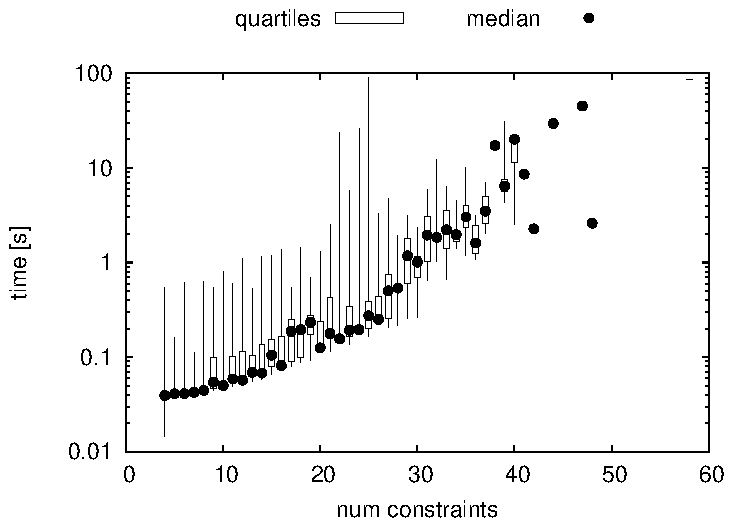
\includegraphics[width=8.5cm]{figures/plot_latte.pdf} \\
\caption{LattE benchmarks}
\label{fig:bench_latte}
\end{figure}
\fi

\section{Implementation and experiments}
\label{sec:impl}

We implemented an interpreter for the language based on the
probabilistic polyhedra powerset domain. The manipulations of
polyhedra are done using the PPL \cite{parma}. Size calculations are
done using the LattE \cite{latte}. LattE is also
used for the integer linear programming problem involved in the
abstract forget operation. The interpreter itself is written in OCaml.
We conducted several experiments on a Mac Pro with two 2.26 GHz
quad-core Xeon processors using 16 GB of RAM and running OS X v10.6.7.
While many of the abstract operations distribute over the set of
probabilistic polyhedra and thus could be parallelized, our
implementation is currently single-threaded.

\fref{fig:plots_bday}(a) illustrates the result of running the query
given in Example~\ref{ex:bday} (Section~\ref{sec:overview}) using our
implementation and one using Probabilistic
Scheme~\cite{radul07probscheme}, which is capable of sound probability
estimation after partial enumeration.  Each $\times$ plots
prob-scheme's maximum probability value (the y axis)---that is, the
probability it assigns to the most likely secret state---when given a
varying amount of time for sampling (the x axis).  We can see the
precision improves steadily until it reaches the exact value of 1/259
at around 17 seconds. Each $+$ plots our implementation's maximum
probability value when given an increasing number of probabilistic
polyhedra; with a polyhedral bound of 2 (or more), we obtain the exact
value in less than 3 seconds. The timing measurements are taken to be
the medians of 12 runs. The advantage of our approach is more evident
in \fref{fig:plots_bday}(b) where we use the same program but allow
$\var{byear}$ to span 1910 to 2010 rather than 1956 to 1992. In this
case prob-scheme makes little progress even after a minute, and
eventually runs out of memory.  Our approach, however, is unaffected
by this larger state space and produces the exact maximum belief in
around 3 seconds when using only 2 probabilistic polyhedra.

\ifacita

\fref{fig:plots_bday}(c) shows the result of assessing the special
query (Example~\ref{ex:specyear}) with initial belief matching that
following the first birthday query.  Each point is the number of
polyhedra allowed.  The result shows that more complex queries, ones
with many disjunctions, slow our approach and reduce the precision of
the maximum probability. The example requires 36 polyhedra for exact
calculations though as little as 3 produce probabilities near
exact. Note that the precision does not increase monotonically with
the number of polyhedra---in some cases more polyhedra leads to a less
precise result.  We conjecture that the occasional worsening of the
precision with increase in the number of allowable polyhedra is due to
an overly simple means of deciding which polyhedra to merge when
performing abstract simplification, a conjecture we plan to
investigate.

\else
\fref{fig:plots_bday}(c) shows the result of our implementation
assessing the special query (Example~\ref{ex:specyear}) with initial
belief matching that following the first birthday query.  Each plotted
point is the number of polyhedra allowed.  The result demonstrates
that more complex queries, specifically ones with many disjunctions in
their conditionals, not only slow our approach, but also reduce the
precision of the maximum probability value. The example requires 36
polyhedra for exact calculations though as little as 3 produce
probabilities near exact. Note that the precision does not increase
monotonically with the number of polyhedra---in some cases more
polyhedra leads to a less precise result.  We conjecture
that the occasional worsening of the precision with increase in the
number of allowable polyhedra is due to an overly simple means of
deciding which polyhedra to merge when performing abstract
simplification; we plan to investigate this issue in future work.
\fi

\iffull

Table~\ref{fig:bench_table} tabulates details for the example programs
along three other queries we developed based on advertising scenarios;
these queries are described in the Appendix~\ref{appendix:queries}. In
each box is the wall clock time for processing (median of 12 runs),
the running time's semi-interquartile range (SIQR), the number of
outliers, which are defined to be the points $ 3\times\text{SIQR} $
below the first quartile or above the third, and the max belief
computed (smaller being more accurate).  Obvious trends are that
running time goes up and max belief goes down as the number of
polyhedra increase, by and large.  There are exceptions to running
time trend, and most are close to the SIQR and so possibly not
statistically significant. The most striking exception is the running
time for poly-size 9 of the ``pizza'' query.  This extreme outlier is
due to a single invocation of LattE on the largest set of constraints
among all the benchmarks performed in the table. We have no good
explanation of how this complex polyhedron arose. \pxm{the previous
  was incorrect, we do know why the outlier exists, fixed.} The only
exceptions to monotonic decrease in max belief are the ``special
queries'', as already discussed.  \mwh{I observe that these are the
  only queries that employ probabilistic choice; any possibility this
  is correlated with the behavior?} \pxm{This might indirectly be the
  cause as it is the only example in which the postbelief is not a
  normalized restriction of the prebelief but I'm not sure how to
  better argue this Mike's hypothesis.}

Investigating the running time results further, we discovered that for
nearly all benchmarks, 95\% or more of the running time is spent in
the LattE counting tool.  The LattE tool exhibits super-exponential
running time in terms of the number of constraints (see
\fref{fig:bench_latte}) over the polyhedra that occur when evaluating
the various queries in Table~\ref{fig:bench_table}. As such, overall
running time is susceptible to the complexity of the polyhedra
involved, even when they are few in number. The merging operation,
while used to keep the number of probabilistic polyhedra below the
required bound, also tends to produce more complex polyhedra. These
observations suggest a great deal of performance improvement can be
gained by simplifying the polyhedra if they become too complex.

\fi

% LocalWords:  bday specyear bigmac

